\documentclass{beamer}
\usepackage{cancel, algpseudocode, hyperref, tikz, venndiagram, centernot}

\title{CS 70 Discussion 14A}
\date{December 4, 2024}

\begin{document}

\frame{\titlepage}

\begin{frame}
    \frametitle{Markov Chains}
    A Markov chain is a sequence of random variables $X_0,X_1,\dots$ that follows the {\bf Markov property}:
    \begin{align*}
        &\mathbb{P}[X_t=x_t|X_0=x_0,\dots,X_{t-1}=x_{t-1}]=\mathbb{P}[X_t=x_t|X_{t-1}=x_{t-1}]\\
        &\phantom{\mathbb{P}[X_t=x_t|X_0=x_0,\dots,X_{t-1}=x_{t-1}]}=P_{x_{t-1},x_t}
    \end{align*}
    This means that the {\bf state} that we are at at a certain time is only dependent on the state we were at at the previous timestep. We refer to $P_{x_{t-1},x_t}$ as a {\bf transition probability} and $P$ as the {\bf transition matrix} ($P$ is a square matrix with the number of rows and number of columns equaling the number of states in our chain). Each row of $P$ also naturally sums to $1$.
\end{frame}

\begin{frame}
    \frametitle{Markov Chains (Cont.)}
    Given the Markov property, you can view a Markov chain as a graph with each node representing a state, and each edge representing the probability of moving from one state to another in a timestep:
    \begin{center}
        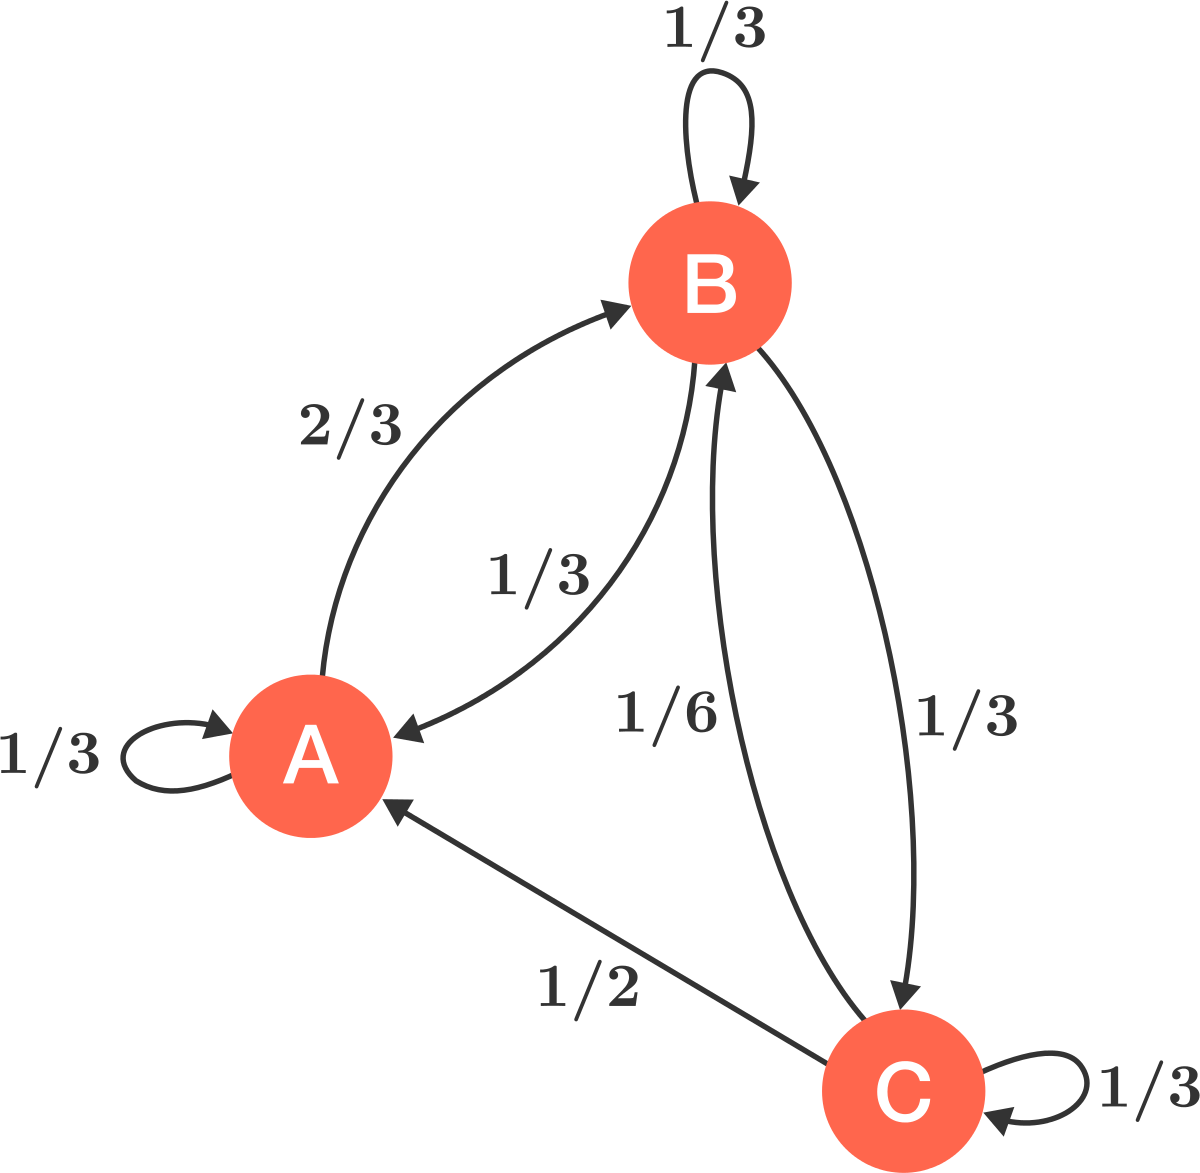
\includegraphics[scale=0.1]{Images/markov-chain.png}
    \end{center}
\end{frame}

\begin{frame}
    \frametitle{Initial Distribution}
    {\bf Problem}: While we have the matrix $P$ to represent our transition probabilities, how do we represent our distribution of states we {\it start} at?\\
    {\bf Solution}: We define $\pi_0$ as the {\bf initial distribution}, where $\mathbb{P}[X_0=x]=\pi_0(x)$. One thing to note is that $\pi_t$ is common notation for the distribution of states we will be at in timestep $t$ (i.e. $\mathbb{P}[X_t=x]=\pi_t(x)$). $\pi$ is a {\it row vector}, and the following property holds for all times $t>0$:
    \begin{align*}
        \pi_t=\pi_{t-1}P=\pi_0 P^t
    \end{align*}
    {\it Note: We are performing matrix multiplication to get $P^t$.}
\end{frame}

\begin{frame}
    \frametitle{Hitting Probability}
    {\bf Problem}: Let's say I start at a state $s$. I want to calculate the probability that I hit state $w$ before I hit state $\ell$. How do I calculate this probability?\\
    {\bf Solution}: We define $\alpha(x)$ as the probability of getting to $w$ before $\ell$ if we are currently at state $x$. We now set-up a system of equations for your Markov chain as follows:
    \begin{align*}
        &\alpha(w)=1\\
        &\alpha(\ell)=0\\
        &(\forall x\neq w,x\neq\ell)\left(\alpha(x)=\sum_{y=1}^n\alpha(y)P_{x,y}\right)
    \end{align*}
    Our desired probability is $\alpha(s)$.
\end{frame}

\begin{frame}
    \frametitle{Hitting Time}
    {\bf Problem}: Let's say I start at state $s$. I want to calculate the expected number of time steps to reach state $w$. How do I calculate this expectation?\\
    {\bf Solution}: We define $\beta(x)$ as the expected time to reach state $w$ starting from $x$. Now, we can set-up the following system of equations for your Markov Chain:
    \begin{align*}
        &\beta(w)=0\\
        &(\forall x\neq w)\left(\beta(x)=1+\sum_{y=1}^n\beta(y)P_{x,y}\right)
    \end{align*}
    Our desired expectation is $\beta(s)$.
\end{frame}

\end{document}
